\documentclass[journal, letterpaper]{IEEEtran}

% some very useful LaTeX packages include:

%\usepackage{cite}      % Written by Donald Arseneau
                        % V1.6 and later of IEEEtran pre-defines the format
                        % of the cite.sty package \cite{} output to follow
                        % that of IEEE. Loading the cite package will
                        % result in citation numbers being automatically
                        % sorted and properly "ranged". i.e.,
                        % [1], [9], [2], [7], [5], [6]
                        % (without using cite.sty)
                        % will become:
                        % [1], [2], [5]--[7], [9] (using cite.sty)
                        % cite.sty's \cite will automatically add leading
                        % space, if needed. Use cite.sty's noadjust option
                        % (cite.sty V3.8 and later) if you want to turn this
                        % off. cite.sty is already installed on most LaTeX
                        % systems. The latest version can be obtained at:
                        % http://www.ctan.org/tex-archive/macros/latex/contrib/supported/cite/

\usepackage{graphicx}   % Written by David Carlisle and Sebastian Rahtz
                        % Required if you want graphics, photos, etc.
                        % graphicx.sty is already installed on most LaTeX
                        % systems. The latest version and documentation can
                        % be obtained at:
                        % http://www.ctan.org/tex-archive/macros/latex/required/graphics/
                        % Another good source of documentation is "Using
                        % Imported Graphics in LaTeX2e" by Keith Reckdahl
                        % which can be found as esplatex.ps and epslatex.pdf
                        % at: http://www.ctan.org/tex-archive/info/

%\usepackage{psfrag}    % Written by Craig Barratt, Michael C. Grant,
                        % and David Carlisle
                        % This package allows you to substitute LaTeX
                        % commands for text in imported EPS graphic files.
                        % In this way, LaTeX symbols can be placed into
                        % graphics that have been generated by other
                        % applications. You must use latex->dvips->ps2pdf
                        % workflow (not direct pdf output from pdflatex) if
                        % you wish to use this capability because it works
                        % via some PostScript tricks. Alternatively, the
                        % graphics could be processed as separate files via
                        % psfrag and dvips, then converted to PDF for
                        % inclusion in the main file which uses pdflatex.
                        % Docs are in "The PSfrag System" by Michael C. Grant
                        % and David Carlisle. There is also some information
                        % about using psfrag in "Using Imported Graphics in
                        % LaTeX2e" by Keith Reckdahl which documents the
                        % graphicx package (see above). The psfrag package
                        % and documentation can be obtained at:
                        % http://www.ctan.org/tex-archive/macros/latex/contrib/supported/psfrag/

%\usepackage{subfigure} % Written by Steven Douglas Cochran
                        % This package makes it easy to put subfigures
                        % in your figures. i.e., "figure 1a and 1b"
                        % Docs are in "Using Imported Graphics in LaTeX2e"
                        % by Keith Reckdahl which also documents the graphicx
                        % package (see above). subfigure.sty is already
                        % installed on most LaTeX systems. The latest version
                        % and documentation can be obtained at:
                        % http://www.ctan.org/tex-archive/macros/latex/contrib/supported/subfigure/

\usepackage{url}        % Written by Donald Arseneau
                        % Provides better support for handling and breaking
                        % URLs. url.sty is already installed on most LaTeX
                        % systems. The latest version can be obtained at:
                        % http://www.ctan.org/tex-archive/macros/latex/contrib/other/misc/
                        % Read the url.sty source comments for usage information.

%\usepackage{stfloats}  % Written by Sigitas Tolusis
                        % Gives LaTeX2e the ability to do double column
                        % floats at the bottom of the page as well as the top.
                        % (e.g., "\begin{figure*}[!b]" is not normally
                        % possible in LaTeX2e). This is an invasive package
                        % which rewrites many portions of the LaTeX2e output
                        % routines. It may not work with other packages that
                        % modify the LaTeX2e output routine and/or with other
                        % versions of LaTeX. The latest version and
                        % documentation can be obtained at:
                        % http://www.ctan.org/tex-archive/macros/latex/contrib/supported/sttools/
                        % Documentation is contained in the stfloats.sty
                        % comments as well as in the presfull.pdf file.
                        % Do not use the stfloats baselinefloat ability as
                        % IEEE does not allow \baselineskip to stretch.
                        % Authors submitting work to the IEEE should note
                        % that IEEE rarely uses double column equations and
                        % that authors should try to avoid such use.
                        % Do not be tempted to use the cuted.sty or
                        % midfloat.sty package (by the same author) as IEEE
                        % does not format its papers in such ways.

\usepackage{amsmath}    % From the American Mathematical Society
                        % A popular package that provides many helpful commands
                        % for dealing with mathematics. Note that the AMSmath
                        % package sets \interdisplaylinepenalty to 10000 thus
                        % preventing page breaks from occurring within multiline
                        % equations. Use:
%\interdisplaylinepenalty=2500
                        % after loading amsmath to restore such page breaks
                        % as IEEEtran.cls normally does. amsmath.sty is already
                        % installed on most LaTeX systems. The latest version
                        % and documentation can be obtained at:
                        % http://www.ctan.org/tex-archive/macros/latex/required/amslatex/math/



% Other popular packages for formatting tables and equations include:

%\usepackage{array}
% Frank Mittelbach's and David Carlisle's array.sty which improves the
% LaTeX2e array and tabular environments to provide better appearances and
% additional user controls. array.sty is already installed on most systems.
% The latest version and documentation can be obtained at:
% http://www.ctan.org/tex-archive/macros/latex/required/tools/

% V1.6 of IEEEtran contains the IEEEeqnarray family of commands that can
% be used to generate multiline equations as well as matrices, tables, etc.

% Also of notable interest:
% Scott Pakin's eqparbox package for creating (automatically sized) equal
% width boxes. Available:
% http://www.ctan.org/tex-archive/macros/latex/contrib/supported/eqparbox/

% *** Do not adjust lengths that control margins, column widths, etc. ***
% *** Do not use packages that alter fonts (such as pslatex).         ***
% There should be no need to do such things with IEEEtran.cls V1.6 and later.
\usepackage{multirow}
% tabularx allows manual tweaking of column width
\usepackage{tabularx}
% longtable does better format for tables that span pages
\usepackage{longtable}
\usepackage{graphicx}
\usepackage{float}
\usepackage{amsmath}
\usepackage{multicol}
\usepackage{hyperref}
% Your document starts here!
\begin{document}

% Define document title and author
	\title{\textbf{Ind-Cap}}
	\author{Hanzhi Yang \\ yang1118@purdue.edu}
	%\thanks{Advisor: Dipl.--Ing.~Firstname Lastname, Lehrstuhl f\"ur Nachrichtentechnik, TUM, WS 2050/2051.}}
	%\markboth{Hauptseminar Digitale Kommunikationssysteme}{}
	\maketitle

% Write abstract here
\begin{abstract}
	Capacitors and Inductors are essential to the operation of analog filters and power electronics. Capacitors are frequently used to store charge in case of a sudden inrush of current draw, and inductors can be used to filter out high frequency noise in a power cable. This lab include four experiments: \textit{building resistors/ capacitors/inductors}, \textit{current and voltage measurements of inductors}, \textit{current and voltage measurements of capacitors}, and \textit{capacitor voltage divider}
\end{abstract}

% Each section begins with a \section{title} command
\section{\textbf{Introduction}}
	% \PARstart{}{} creates a tall first letter for this first paragraph
	% \PARstart{T}{his} section introduces the topic and leads the reader on to the main part.
    \subsection{Objectives}
    	\begin{itemize}
        	\item Use LCR to measure inductance, capacitance, and resistance
            \item Build inductor, resistor, and capacitor with materials provided by instructors
            \item Test the quantities of the self-made components
        \end{itemize}
    \subsection{Equipment}
    	\begin{multicols}{2}
          \begin{flushleft}
    		\begin{itemize}
            \item Digital Multimeter (DMM)
            \item Function Generator (FG)
            \item LCR Meter (LCR)
            \item Oscilloscope (scope)
            \item Resistor
            \item Inductor
            \item Capacitor
            \item Cables
            \end{itemize}
          \end{flushleft}
    	\end{multicols}
    	
% Main Part
\section{\textbf{Task 1: Building Resistors, Capacitors and Inductors}}
	\subsection{Objective}
    	\begin{itemize}
    		\item Use LCR to test the self-made resistor, capacitor, and inductor
    		\end{itemize}
    \subsection{Design}
    	\begin{itemize}
    	\item Circuit Design
    	\end{itemize}
        \begin{figure}[!hbt]
		% Center the figure.
		\begin{center}
		% Include the eps file, scale it such that it's width equals the column width. You can also put width=8cm for example...
		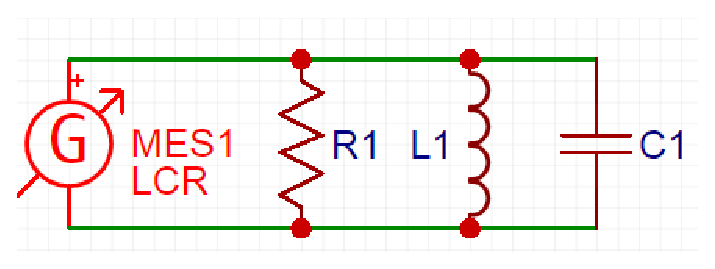
\includegraphics[width=\columnwidth]{l7_1}
		% Create a subtitle for the figure.
		\caption{Circuit Design for Task 1}
		% Define the label of the figure. It's good to use 'fig:title', so you know that the label belongs to a figure.
		\label{fig:l7_1}
		\end{center}
	\end{figure}
    \newpage
    \begin{itemize}
		\item Calculation
          \begin{flushleft}
              \begin{multicols}{2}
                  \begin{itemize}
                      \item $R = \rho\frac{L}{A}$
                      \item $C = \epsilon\frac{A}{d}$
                      \item $L_{coil} = N^{2}\mu_{0}\mu_{r}R[ln(\frac{8R}{r})-2]$
                  \end{itemize}
              \end{multicols}
          \end{flushleft}
    \end{itemize}
    \subsection{Procedures}
    	\begin{enumerate}
        	\item Estimate the resistance across a piece of pencil lead \footnote{Graphite has a resistivity on the order of $3\cdot
10^{-5}\Omega$ m}
            \item Use LCR to measure the resistance of the piece of pencil lead; compute the error (\textit{see Table 1})
            \item Estimate the capacitance of a capacitor built with two metal plates separated by a single sheet of printer paper
            \item Build the capacitor and use LCR to measure the capacitance; compute the error (\textit{see Table 1})
            \item Estimate the inductance of a 20 turn inductor with a diameter of 5mm
            \item Build the inductor and use an LCR to measure the inductance; compute the error (\textit{see Table 1})
        \end{enumerate}
    \subsection{Results}
    	% This is how you define a table: the [!hbt] means that LaTeX is forced (by the !) to place the table exactly here (by h), or if that doesnt work because of a pagebreak or so, it tries to place the table to the bottom of the page (by b) or the top (by t).
	\begin{table}[!hbt]
		% Center the table
		\begin{center}
		% Title of the table
		\caption{LCR Readings}
		\label{tab:LCRReadings}
		% Table itself: here we have two columns which are centered and have lines to the left, right and in the middle: |c|c|
		\begin{tabular}{|c|c|c|c|}
			% To create a horizontal line, type \hline
			\hline
			% To end a column type &
			% For a linebreak type \\
			 $ $  & Computed Value & Measured & \%Error\\
			\hline
			Resistor & 7.0158$\Omega$ &1.1835 $\Omega$ & 83\%\\
			\hline
\(\)		Capacitor &60.87nF & 65.4nF & 7.44\%\\
			\hline
			Inductor & 0.702mH & 0.759mH & 8.1\%\\
			\hline
		\end{tabular}
		\end{center}
	\end{table}
    
    \subsection{Evaluations}
    \begin{enumerate}
    \item The percent error of the resistance is so large that it can be concluded that the resistivity of the tested pencil lead is not as the data provided. With the equation $R = \rho\frac{L}{A}$ the resistivity can be computed to be $1.59\cdot10^{-5}\Omega m$
%				\item The large percent error of the inductance indicates that the screwdriver in the 207 kits is not purely made of steel which should have a relative permeability of 2000; in the experiment the relative permeability of the material of the screwdriver is computed to be 
    \end{enumerate}
    \subsection{Conclusion}
	% LaTeX takes complete care of your document layout ...
	%The presentation's content is summarized in the report in 4~pages.
	% ... but you can insert a line break manually with two backslashes, if needed: \\
	%The author should fill, but not exceed, this space. \\
	%The report should be a self-contained report, so that it can be understood without studying additional literature.
    			The measured values have a large difference from the computed values. Therefore, the constant of the materials need to be tested for future experiments. Also, some errors on the manipulation may increase errors on the measured values. 

\section{\textbf{Task 2: Current and Voltage Measurements of Inductors}}
	\subsection{Objective}
    	\begin{itemize}
    		\item Use scope to test the current and voltage across the self-made inductor
    	\end{itemize}
    \subsection{Design}

        \begin{itemize}
        \item Calculation
        	\begin{itemize}
        	\item $V = L\frac{dI}{dt}$
        	\end{itemize}
        \end{itemize}
            	\begin{itemize}
    	\item Circuit Design      \begin{figure}[!hbt]
        	\begin{center}
		% Include the eps file, scale it such that it's width equals the column width. You can also put width=8cm for example...
				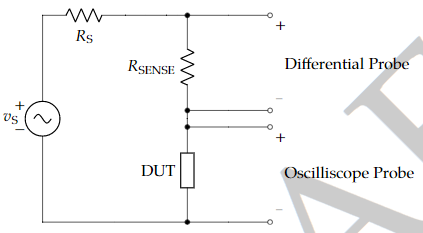
\includegraphics[width=\columnwidth]{l7_2}
		% Create a subtitle for the figure.
				\caption{Circuit Design for Task 2}
		% Define the label of the figure. It's good to use 'fig:title', so you know that the label belongs to a figure.
				\label{fig:l7_2}
			\end{center}
        \end{figure}
    	\end{itemize}
    \subsection{Procedures}
    	\begin{enumerate}
    	\item Build the test circuit (see \textit{Fig 2}) with $R_{SENSE}=100\Omega$ and the inductor in task 1
        \item Use FG to generate a sine wave with peak-to-peak voltage 20V and frequency 100kHz; measure the voltage across inductor and $R_{SENSE}$
        \item Compute the inductance of the inductor and the error
        \item Repeat using a 1mH inductor with $R_{SENSE}=1K\Omega$
    	\end{enumerate}
    \subsection{Results}
    	\begin{enumerate}
    	\item The voltage across the inductor and the resistor in the case of $R_{SENSE}=100\Omega$
    				\begin{itemize}
    				\item $V_L = 0.06cos(2\pi100000t)$
    				\item $V_R = 13.3sin(2\pi100000t)$
                    \end{itemize}
\item The voltage across the inductor and the resistor in the case of $R_{SENSE} = 1k\Omega$
		\begin{enumerate}
		\item $V_L = 0.0086cos(2\pi100000t)$
\item $V_R = 19.1sin(2\pi100000t)$
		\end{enumerate}
    \end{enumerate}

    \subsection{Evaluations}
    \begin{enumerate}
    \item To compute the current, based on the equation $V = L\frac{dI}{dt}$ and $I = \frac{V}{R}$ , the current across the resistor is $$I_R = \frac{V_R}{R_{SENSE}} = \frac{13.3sin(2\pi100000t)}{100}$$ and the voltage across the inductor is $$V_L = L\frac{dI_R}{dt} = L\cdot0.133cos(2\pi100000t)2\pi100000$$ and $$V_L = 0.06cos(2\pi100000t)$$ $$0.06 = 0.133L\cdot2\pi100000$$$$L = 0.845mH$$
\item The error is 20.4\%
\item With $R_{SENSE} = 1K\Omega$, $L = 0.718mH$, and the error is 2.3\%

    \end{enumerate}
    \subsection{Conclusion}
    The test result has a large error compared with the computed value; this may be caused by that the coil for inductor is not winded tightly around the screwdriver and thus there is air between the screwdriver and the coil which would caused to the measured value to be inaccurate. 
\section{\textbf{Task 3: Current and Voltage Measurements of Capacitors}}
	\subsection{Obejctive}
    	\begin{itemize}
    		\item Use scope to test the current and voltage across the self-made capacitor
    	\end{itemize}
	\subsection{Design}
    	\begin{itemize}
    		\item Circuit Design
    	\end{itemize}
        \begin{figure}[!hbt]
        	\begin{center}
        		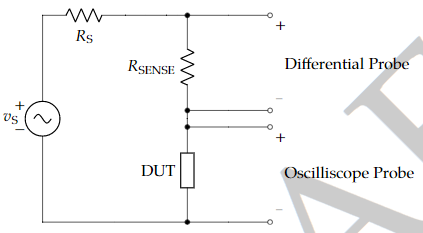
\includegraphics[width=\columnwidth]{l7_2}
                \caption{Circuit Design for Task 3}
                \label{fig:l7_3}
        	\end{center}
        \end{figure}
        \begin{itemize}
        \item Calculation
        	\begin{itemize}
        	\item $I = C\frac{dV}{dt}$
        	\end{itemize}
        \end{itemize}
    \subsection{Procedures}
    	\begin{enumerate}
    	\item Build the test circuit (\textit{see Fig 3}) with $R_{SENSE} = 1k\Omega$ and the capacitor in Task 1
        \item Use FG to generate a sine wave with 10V peak-to-peak voltage and 100kHz frequency; measure the voltage across the capacitor and $R_{SENSE}$
        \item Compute the capacitance of the capacitor and the error
        \item Repeat using one 10nF capacitor, then using two 10nF in parallel, and then in series
    	\end{enumerate}
    \subsection{Results}
\begin{enumerate}
\item The voltage in the experiment with the self-made capacitor is \begin{itemize}
\item $V_R = 9.6cos(2\pi100000t)$
\item $V_C = 0.275sin(2\pi100000t)$
\end{itemize}
\item The voltage in the experiment with one 10nF capacitor is \begin{itemize}
\item $V_R = 9.6cos(2\pi100000t)$
\item $V_C = 1.35sin(2\pi100000t)$
\end{itemize}
\newpage
\item The voltage in the experiment with two 10nF capacitors in parallel is \begin{itemize}
\item $V_R = 9.6cos(2\pi100000t)$
\item $V_C = 0.84sin(2\pi100000t)$
\end{itemize}
\item The voltage int he experiment with two 10nF capacitors in series is \begin{itemize}
\item $V_R = 9.6cos(2\pi100000t)$
\item $V_C = 3.40sin(2\pi100000t)$
\end{itemize}
\end{enumerate}

    \subsection{Evaluations}
    \begin{enumerate}
    \item To compute the capacitance, according to the equations $I = C\frac{dV}{dt}$ and $I = \frac{V}{R}$ , $$i_C = \frac{V_R}{R} = \frac{V_R}{1000}$$and $$i_C = C\frac{dV_C}{dt}$$ therefore, $$\frac{V_R}{1000} = V\frac{dV_C}{dt}$$ $$C\cdot0.275\cdot(2\pi100000t)2\pi100000 = \frac{1}{1000}\cdot9.6cos(2\pi100000t)$$thus $$C = 55.6nF$$ The error is 8.66\%
\item With the same procedures of computation, the capacitance in the experiment with one 10nF capacitor is equal to 11.3nF, and the error is 13\%
\item The capacitance in the experiment with two 10nF capacitors in parallel is 18.2nF, and the error is 9\%
\item The capacitance in the experiment with two 10nF capacitors in series is 4.5nF, and the error is 10\%
        \end{enumerate}
    \subsection{Conclusion}
	The result capacitance of capacitors in parallel is $C_{result} = C_1 + C_2$. The results capacitance of capacitors in series is $\frac{1}{C_{result}} = \frac{1}{C_1} + \frac{1}{C_2}$ . 
\section{\textbf{Task 4: Capacitor Voltage Divider}}
	\subsection{Objective}
    \begin{itemize}
    \item Use scope to test the capacitor voltage divider
    \end{itemize}
    
\newpage
    \subsection{Design}
    \begin{itemize}
    \item Circuit Design
    \end{itemize}
    \begin{figure}[!hbt]
    	\begin{center}
    		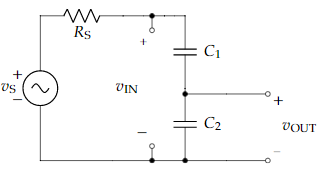
\includegraphics[width=\columnwidth]{l7_3}
            \caption{Circuit Design for Task 4}
            \label{fig:l7_4}
    	\end{center}
    \end{figure}
%	\begin{itemize}
%	\item Calculation
%    	\begin{itemize}
%    	\item 
%    	\end{itemize}
%	\end{itemize}
	\subsection{Procedures}
    \begin{enumerate}
    \item Build the test circuit (\textit{see Fig 4}) with $C_1 = 0.47\mu F $ and $ C_2 = 0.1\mu F$
    \item Use FG to generate a sine wave with 5V peak-to-peak voltage and 10kHz frequency
    \item Connect scope's input 1 to $v_{IN}$ and input 2 to $v_{OUT}$; plot the two signals on the same screen (\textit{see Fig 5})
    \item Swap $C_1 and C_2$; plot the new signals (\textit{see Fig 6})
    \item Change the frequency of FG; observe the attenuation ratio
    \item Change the FG to DC mode and sweep the voltage from 0V to 10V with a step of 1V; observe the signals (\textit{see Fig 7, Table 3})
    \end{enumerate}
	\subsection{Results}
    \begin{figure}[!hbt]
    \begin{center}
    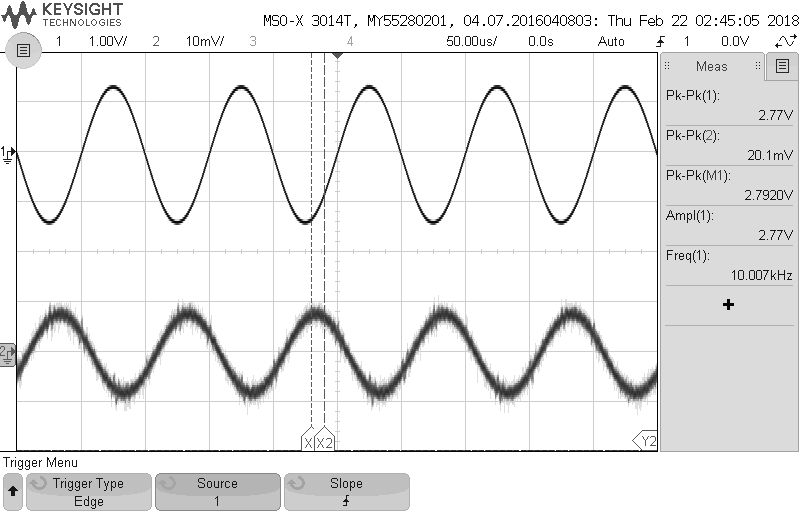
\includegraphics[width=\columnwidth]{scope_16}
    \caption{Voltage Input and Output}
    \label{fig:scope_17}
    \end{center}
    \end{figure}
    \begin{figure}[!hbt]
    \begin{center}
    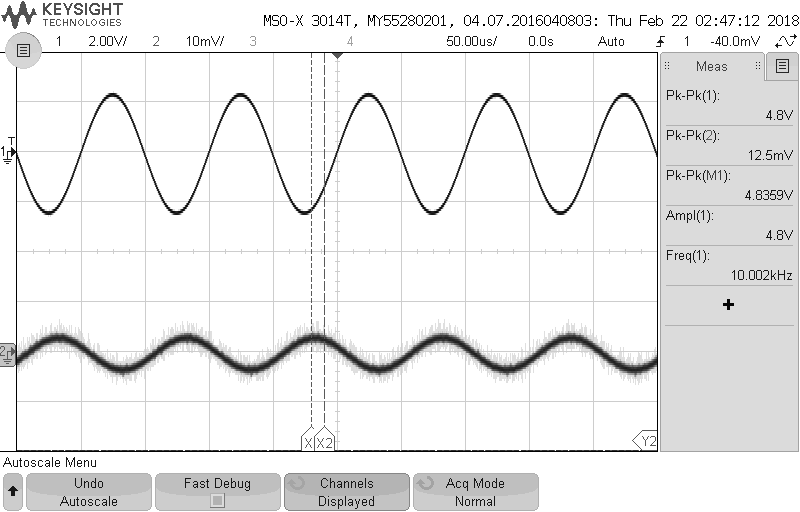
\includegraphics[width=\columnwidth]{scope_17}
    \caption{Voltage Output and Input}
    \label{fig:scope_18}
    \end{center}
    \end{figure}
        \begin{figure}[!hbt]
    \begin{center}
    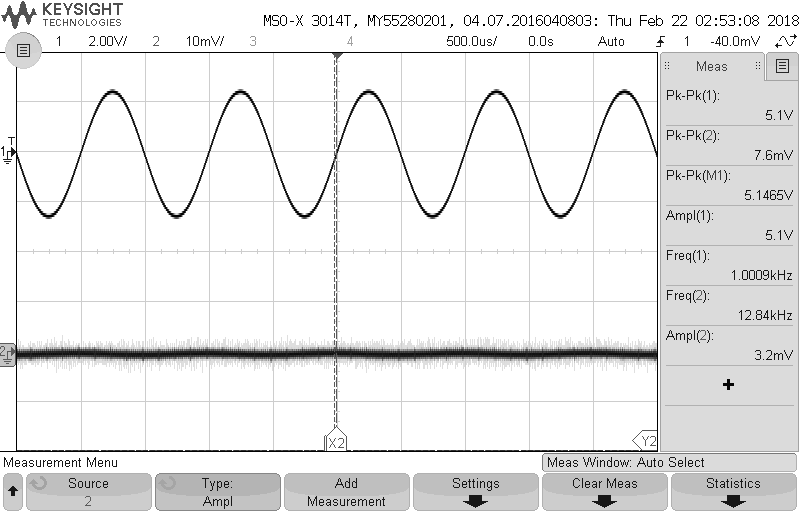
\includegraphics[width=\columnwidth]{scope_19}
    \caption{Change the Frequency form 10KHz to 1KHz}
    \label{fig:scope_19}
    \end{center}
    \end{figure}
	\begin{table}[!hbt]
		% Center the table
		\begin{center}
		% Title of the table
		\caption{Voltage Input and Output with Variable Voltage Source}
		\label{tab:VIOVVS}
		\begin{tabular}{|c|c|c|}
			% To create a horizontal line, type \hline
			\hline
			% To end a column type &
			% For a linebreak type \\
			 \textbf{$V_S$} & \textbf{$V_{IN}$} & \textbf{$V_{OUT}$}\\
			\hline
			0v &3.2mv & 3.2mv\\
			\hline
\(\)	1v &3.2mv & 3.2mv\\
			\hline
			2v &3.2mv & 3.2mv\\
			\hline
            3v &3.2mv & 3.2mv\\
			\hline
            4v &3.2mv & 3.2mv\\
			\hline
            5v &3.2mv & 3.2mv\\
			\hline
            6v &3.2mv & 3.2mv\\
			\hline
            7v &3.2mv & 3.2mv\\
			\hline
            8v &3.2mv & 3.2mv\\
			\hline
            9v &3.2mv & 3.2mv\\
			\hline
            10v &3.2mv & 3.2mv\\
			\hline
            
		\end{tabular}
		\end{center}
        \end{table}
        \newpage
\subsection{Evaluations}
    \begin{enumerate}
    \item After $C_1$ and $C_2$ were swapped, the signal plot (\textit{see Fig 6}), compared with the original plot (\textit{see Fig 5}), became more intensive as it can be viewed in the two plots with same time scale. Because the capacitance of $C_2$ is larger than $C_1$, the voltage across $C_1$ in the second plot is smaller than that across $C_2$ in the first plot while the $V_{IN}$ remains the same
\item Changing the frequency of FG does not necessarily affect the attenuation ratio since in this case the only quantity changed is the frequency and thus the voltage ratio remains the same
\item If FG generates DC voltage to the circuit, the circuit does not work like a voltage divider since in a DC circuit, capacitors are like open circuit when fully charged; therefore, the voltage across the capacitor in this experiment is small
    \end{enumerate}
    \subsection{Conclusion}
		Capacitors can be used as voltage dividers in a AC circuit but they would be work in a DC circuit. 
\end{document}